% -- Iniciando o documento --
\documentclass[
	12pt,		% Tamanho da fonte
	a4paper,	% Tamanho do papel
	english,	% Idioma adicional
	brazil,		% Idioma principal
	openright,	% Capitulos começam em pag impar
	oneside		% Apenas 1 página por folha
	]{abntex2}

\usepackage{lmodern}			% Usa a fonte Latin Modern
\usepackage[T1]{fontenc}		% Selecao de codigos de fonte.
\usepackage[utf8]{inputenc}		% Codificacao do documento
\usepackage{lastpage}			% Usado pela Ficha catalográfica
\usepackage{indentfirst}		% Identa o primeiro parágrafo de cada seção.
\usepackage{color}				% Controle das cores
\usepackage{xcolor}
\usepackage{graphicx}			% Inclusão de gráficos
\usepackage{microtype} 			% para melhorias de justificação
\usepackage{lipsum}				% para geração de dummy text
\usepackage{geometry}			% para alteração no layout das páginas
\usepackage{lscape}             % colocar páginas na horizontal compativel com longtable e supertabular.
\usepackage{bookmark}
\usepackage{caption}            % adiciona \caption*{d} para criar fontes em imagens.
\usepackage{float}				% para uso no posicionamento de imagens
\usepackage{pdfpages}
\usepackage{minibox}
\usepackage{listings}
\usepackage{multirow}           % Habilita o Merge de celulas na table

% ---
% Alterações no modelo original da abnTex2
% ---
% Impressão da Capa
\renewcommand{\imprimircapa}{%
  \begin{capa}%
    \center
    \ABNTEXchapterfont\large\imprimirinstituicao\\
    \vspace{5cm}
    \imprimirautor

    \vfill
    \begin{center}
    \ABNTEXchapterfont\bfseries\LARGE\imprimirtitulo
    \end{center}
    \vfill

    \large\imprimirlocal

    \large\imprimirdata

    \vspace*{1cm}
  \end{capa}
}
% ---
% Alteração na assinatura dos componentes da banca
\setlength{\ABNTEXsignwidth}{10cm}

\geometry{
 a4paper,
 bottom=2cm,
 top=3cm,
 left=3cm,
 right=2cm
}

% ---
% Configura layout para elementos textuais
\renewcommand{\textual}{%
  \pagestyle{plain}%abntheadings
  %\nouppercaseheads%
  \bookmarksetup{startatroot}%
  \pagenumbering{arabic}
}

\renewcommand{\pretextual}{%
  \pagestyle{plain}
  \pagenumbering{Roman}
}

%%% -----
%%% Formato de cabeçalho/rodapé romano nos elementos pré-textuais
%%% -----

%% Novo estilo
\makepagestyle{estilo_pretextual} %%% escolha um nome
  %\makeevenhead{estilo_pretextual}{}{}{\ABNTEXfontereduzida \textbf \thepage}
  \makeoddhead{estilo_pretextual}{}{}{\ABNTEXfontereduzida \textbf \thepage}

%% Customiza comando \pretextual
\renewcommand{\pretextual}{
  \pagenumbering{Roman} %%% ou \pagenumbering{Roman}
  \aliaspagestyle{chapter}{estilo_pretextual}% customizing chapter pagestyle
  \pagestyle{estilo_pretextual}
  \aliaspagestyle{cleared}{empty}
  \aliaspagestyle{part}{estilo_pretextual}
}

% ---
% Ajusta a marca \textual para que a numeração volte a ser arábica
% nos elementos textuais
\let\oldtextual\textual        % copia o comando \textual anterior para \oldtextual
\renewcommand{\textual}{%
  \pagestyle{plain}%abntheadings
  %\nouppercaseheads%
  \aliaspagestyle{chapter}{plain}
  \bookmarksetup{startatroot}%
  \pagenumbering{arabic}
}
% ---

\makeatletter
\renewcommand*{\ps@plain}{%
  \let\@mkboth\@gobbletwo
  \let\@oddhead\@empty
  \def\@oddfoot{%
    \reset@font
    \hfil
    \thepage
    % \hfil % removed for aligning to the right
  }%
  \let\@evenhead\@empty
  \let\@evenfoot\@oddfoot
}
\makeatother

% ---
% Pacotes de citações
% ---
\usepackage[brazilian, hyperpageref]{backref}	 % Paginas com as citações na bibl
\usepackage[alf]{abntex2cite}	% Citações padrão ABNT



% ---
% CONFIGURAÇÕES DE PACOTES
% ---

% ---
% Configurações do pacote backref
% Usado sem a opção hyperpageref de backref
\renewcommand{\backrefpagesname}{Citado na(s) página(s):~}
% Texto padrão antes do número das páginas
\renewcommand{\backref}{}
% Define os textos da citação
\renewcommand*{\backrefalt}[4]{
	\ifcase #1 %
		Nenhuma citação no texto.%
	\or
		Citado na página #2.%
	\else
		Citado #1 vezes nas páginas #2.%
	\fi}%
% ---

% ---
% Informações de dados para CAPA e FOLHA DE ROSTO
% ---
\titulo{Criação de componentes para o framework Esfinge Gamification}

\autor{Weslei Luiz de Paula Pinto}
\local{São José dos Campos}
\data{\the\year}

\orientador{Me. Gerson da Penha Neto}
\coorientador{Dr. Eduardo Martins Guerra}

\instituicao{%
  FACULDADE DE TECNOLOGIA DE SÃO JOSÉ DOS CAMPOS
  \par
  FATEC PROFESSOR JESSEN VIDAL}

\tipotrabalho{Trabalho de Graduação}

\newcommand{\disciplina}{Análise e Desenvolvimento de Sistemas}

\preambulo{Trabalho de Graduação apresentado à Faculdade de Tecnologia São José dos Campos, como parte dos requisitos necessários para a obtenção do título de Tecnólogo em \disciplina.}

% Comandos para a folha de catalogacao
\newcommand{\cursoRef}{Curso de Tecnologia em \disciplina}
\newcommand{\instituicaoRef}{FATEC de S\~ao Jos\'e dos Campos: Professor Jessen Vidal}
\newcommand{\sobrenomeRef}{Sobrenome referência}
\newcommand{\nomeRef}{Nomes referência}
\newcommand{\rgRef}{49.979.890-9} % Número do RG

% informações do PDF
\makeatletter
\hypersetup{
     	%pagebackref=true,
		pdftitle={\@title},
		pdfauthor={\@author},
    	pdfsubject={\imprimirpreambulo},
	    pdfcreator={LaTeX with abnTeX2},
		pdfkeywords={abnt}{latex}{abntex}{abntex2}{trabalho acadêmico},
		colorlinks=true,       		% false: boxed links; true: colored links
    	linkcolor=blue,          	% color of internal links
    	citecolor=blue,        		% color of links to bibliography
    	filecolor=magenta,      		% color of file links
		urlcolor=blue,
		bookmarksdepth=4
}
\makeatother

% ---
% Espaçamentos entre linhas e parágrafos
% ---
\setlength{\parindent}{1.3cm} % Tamanho do parágrafo

% Controle do espaçamento entre um parágrafo e outro:
\setlength{\parskip}{0.2cm}  % tente também \onelineskip

% ---
% compila o indice
% ---
\makeindex
% ---

% ----
% Início do documento
% ----
\begin{document}
\pretextual
\selectlanguage{brazil}
\frenchspacing % Retira espaço extra obsoleto entre as frases

% ---
% Configuring all citations
\citeoption{abnt-etal-list=0}
\citeoption{abnt-last-names=abnt}
\citeoption{abnt-full-initials=yes}
% ---

% ---
% Configuring listing code
% See references on internet
% ---
\lstdefinestyle{customc}{
  belowcaptionskip=1\baselineskip,
  breaklines=true,
  %frame=L,
  xleftmargin=\parindent,
  language=C,
  numbers=left,
  showstringspaces=false,
  frame=single,
  basicstyle=\footnotesize\ttfamily,
  keywordstyle=\bfseries\color{green!40!black},
  commentstyle=\itshape\color{purple!40!black},
  identifierstyle=\color{blue},
  stringstyle=\color{orange},
}

\lstset{escapechar=@,style=customc}

% ---

% ---
% Capa
% ---
\imprimircapa
% ---

% ---
% Folha de rosto
% (o * indica que haverá a ficha bibliográfica)
% ---
\thispagestyle{empty}
\imprimirfolhaderosto
% ---

% ---
% Inserir a ficha bibliografica
% ---

\begin{fichacatalografica}
    %\includepdf{./testFicha}
    %%%%%%%%%%%%%
%
% Do not Edit this file!
%
%%%%%%%%%%%%%

\noindent\textbf{Dados Internacionais de Catalogação-na-Publicação (CIP)\\
Divisão de Informação e Documentação}


\noindent\framebox[\textwidth]{%
  % horizonal margin: 10\unitlength
  \parbox{400\unitlength}{%
    \sobrenomeRef, \nomeRef \\
    \imprimirtitulo \\
    \imprimirlocal, \the\year \\
    \pageref{LastPage}f. \\
    \\ \\
    \imprimirtipotrabalho\ -- \cursoRef \\
    \instituicaoRef, \the\year \\
    Orientador: \imprimirorientador \\
    Coorientador: \imprimircoorientador \\
    \\
    \'Areas de Conhecimento. I. Faculdade de Tecnologia. \instituicaoRef. Divis\~ao de Informa\c{c}\~ao e Documenta\c{c}\~ao. II. \imprimirtitulo
  }%
}\\
\parbox{400\unitlength}{
\vspace*{2cm}

\textbf{REFER\^ENCIA BIBLIGR\'AFICA ---} \\ \\
\sobrenomeRef, \nomeRef. \imprimirtitulo \the\year. \pageref{LastPage}f. \imprimirtipotrabalho\ -- \instituicaoRef.

\vspace*{3cm}
\textbf{CESS\~AO DE DIREITOS ---}\\ \\
NOME DO AUTOR: \imprimirautor \\
T\'ITULO DO TRABALHO: \imprimirtitulo \\
TIPO DO TRABALHO/ANO: \imprimirtipotrabalho/\the\year \\

\vspace*{2cm}
É concedida à FATEC de São José dos Campos: Professor Jessen Vidal permissão para reproduzir cópias deste Trabalho e para emprestar ou vender cópias somente para propósitos acadêmicos e científicos. O autor reserva outros direitos de publicação e nenhuma parte deste Trabalho pode ser reproduzida sem a autorização do autor.\\

\vspace*{2cm}
\noindent\rule{7cm}{0.4pt}\\
\imprimirautor \\RG: \rgRef
}

\end{fichacatalografica}

% ---
% Folha de aprovação
% ---

% Descomentar para imprimir a folha
\begin{folhadeaprovacao}

  \begin{center}
    {\ABNTEXchapterfont\large\imprimirautor}

    \vspace*{\fill}\vspace*{\fill}
    \begin{center}
      \ABNTEXchapterfont\bfseries\Large\imprimirtitulo
    \end{center}
    \vspace*{\fill}

    \hspace{.45\textwidth}
    \begin{minipage}{.5\textwidth}
        \imprimirpreambulo
    \end{minipage}%
    \vspace*{\fill}

    Composição da Banca
   \end{center}

   \assinatura{\textbf{\imprimirorientador} \\ Orientador\\}
   \begin{center}
   {\textbf{\imprimircoorientador} \\ Coorientador\\\vspace*{0.5cm}}
   {\textbf{Nome do Professor 1} \\ Professor Convidado\\\vspace*{0.5cm}}
   {\textbf{Nome do Professor 2} \\ Professor Convidado\\\vspace*{0.5cm}}

\end{center}   
   \begin{center}
    \vspace*{0.5cm}
    {\large\imprimirlocal}
    \par
    {\large\imprimirdata}
    \vspace*{1cm}
  \end{center}

\end{folhadeaprovacao}


% Descomentar quando o arquivo folhaAprov.pdf estiver no diretorio raiz
%\includepdf[]{folhaAprov.pdf}
% ---

% ---
% Dedicatória
% ---
\begin{dedicatoria}
   \vspace*{\fill}
   \centering
   \noindent
   \textit{Alguma dedicatoria; frase bonita; e entre outros}
   \vspace*{\fill}
\end{dedicatoria}
% ---

% ---
% Agradecimentos
% ---
\begin{agradecimentos}
\par Agradecimentos do TG.
\end{agradecimentos}
% ---

% ---
% Epigrafe
% ---
\begin{epigrafe}
    \vspace*{\fill}
    \begin{flushright}
        \textit{“Epigrafe, citar alguma frase de outra pessoa que tenha rela\~c\~ao com o TG”\\
        (Seu nome)}
    \end{flushright}
\end{epigrafe}

% ---

% ---
% RESUMOS
% ---
% resumo em português
\setlength{\absparsep}{18pt} % ajusta o espaçamento dos parágrafos do resumo
% --- resumo em português ---
\begin{resumo}

    %Problema. Objetivo. O que fez para cumprir o objetivo. Resultado.
     Geralmente, jogos que possuem restrições têm os recursos desbloqueados conforme o progresso do personagem ou a consecução de algum objetivo. Aplicações que implementam lógicas de gamificação costumam possuir esta abordagem para condicionar comportamentos em seus usuários a partir de regras de autorização. Restrições de uso aumentam o empenho dos usuários para a obtenção de novas funcionalidades ou recursos. Isto é reconhecido na área da Psicologia Comportamental como reforço negativo \cite{skinner1990behavior}. Atualmente o Esfinge Gamification não possui funcionalidades deste tipo, portanto, este trabalho é motivado pela oportunidade da criação de funcionalidades de autorização baseadas em conquistas existentes no \textit{framework}. Para isto o Esfinge Guardian foi integrado ao Esfinge Gamification, possibilitando a utilização de mecanismos de autorização em aplicações Java a partir da definição de metadados via anotações, para assim, desencadear comportamentos de autorização transparentes na aplicação, seguindo a filosofia dos projetos Esfinge.
     
    \vspace{\onelineskip}
    \noindent
    \textbf{Palavras-chave}: Esfinge Project, Esfinge Gamification, gamificação, autorização, \textit{framework}.
\end{resumo}

% resumo em inglês
\begin{resumo}[Abstract]
    \begin{otherlanguage*}{english}
        Usually, games used O abstract é o resumo da obra em língua estrangeira, que basicamente segue o mesmo conceito e as mesmas regras que o texto em português. Recomenda-se que para o texto do abstract o autor traduza a versão do resumo em português e faça, se necessário, os ajustes referentes à conversão dos idiomas. É importante observar que o título e texto NÃO DEVEM estar em itálico.
	    \vspace{\onelineskip}
	    \noindent
	    \\
	    \textbf{Keywords}: Esfinge Project, Esfinge Gamification, Esfinge Guardian, gamification, authorization, framework.
    \end{otherlanguage*}
\end{resumo}
% ---

% ---
% inserir lista de ilustrações
% ---
\pdfbookmark[0]{\listfigurename}{lof}
\listoffigures*
\cleardoublepage
% ---

% ---
% inserir lista de tabelas
% ---
\pdfbookmark[0]{\listtablename}{lot}
\listoftables*
\cleardoublepage
% ---

% ---
% inserir lista de abreviaturas e siglas
% ---
% Listas de Siglas utilizadas no TG
\begin{siglas}
    \item[FaTeX] \emph{Fatec LaTeX}
    \item[TG] \emph{Trabalho de Gradua\~c\~ao}
\end{siglas}
% ---

% ---
% inserir lista de símbolos
% ---
% Lista de simbolos utilizadas no TG

\begin{simbolos}
    \item[<T>] Convenção de declaração de  tipo genérico
    \item[<?>] Declaração de caractere coringa, do inglês \textit{wildcard}. Utilizado para quando não se sabe o tipo que será recebido
\end{simbolos}
% ---
% ---
% inserir o sumario
% ---
\pdfbookmark[0]{\contentsname}{toc}
\tableofcontents*
\cleardoublepage
% ---

% ----------------------------------------------------------
% ELEMENTOS TEXTUAIS
% ----------------------------------------------------------

\textual

\setcounter{page}{15}
% ---
% Incluindo Capitulo 1 - Introducao
% ---
% ----------------------------------------------------------
% Introdução (exemplo de capítulo sem numeração, mas presente no Sumário)
% ----------------------------------------------------------
\chapter[Introdução]{Introdução}
%\addcontentsline{toc}{chapter}{Introdução}
% ----------------------------------------------------------
\par Este capítulo apresenta a motivação deste trabalho, os objetivos definidos, assim como sua metodologia.

\section{Motivação}

\par Devido ao crescimento do termo gamification nos últimos anos, \cite{groh2012gamification} aplicações com contextos não relacionados a jogos, vem adotando esta metodologia para estimular usuários a realizarem determinados processos. Alguns exemplos de aplicações que utilizam gamification são Duolingo \cite{melo2016eficiencia} e foursquare \cite{huotari2012defining}.

\par Adicionar funcionalidades de gamification à aplicações, aumenta a complexidade do projeto para o desenvolvedor, pois será necessário desenvolver a aplicação em si e os processos que desencadeiam a lógica de gamification baseando-se no fluxo desta aplicação, isto também pode dificultar uma manutenção futura.

\par O trabalho é motivado pela oportunidade de automatização no processo de desenvolvimento de módulos e componentes que aplicam lógicas de gamificação, como troféus, recompensas, pontos ou rankings para determinado usuário definido.
\par Aplicações em diferentes contextos não relacionados a jogos que optem implementar gamificação para cativar ou seus usuários. (complementar)
\par Recomendável a utilização de figuras e/ou tabelas.

\section{Problema}
\par Apresente claramente o seu problema.

% Section Objetivo Geral!
\section{Objetivo Geral}
\par Implementação de novos recursos no framework de gamification dando continuidade no trabalho desenvolvido por Dr. Eduardo Guerra, em conjunto com outros colaboradores do INPE e da UNIFESP. 

% Section Objetivo Especifico!
\section{Objetivo Espec\'ifico}
\par Para a consecução deste objetivo foram estabelecidos os objetivos específicos:
\begin{itemize}
    \item Anotações para persistência dos dados de gamificação;
    \item Anotações para interceptação e captura de eventos relevantes a pontuação;
    \item Controle de acesso baseado em conquistas.
\end{itemize}


% ---

% ---
% Incluindo Capitulo 2 - Fundamentacao Teorica
\chapter{Fundamentação Teórica}
\label{ch:fundamentacao}
\par Neste capítulo ser\~ao fundamentados os conhecimentos b\'asicos para o entendimento do trabalho.


\section{Java}

Java é uma linguagem de programação 

\subsection{Reflection}

\subsection{Annotation}

\section{Sistema}

\subsection{Software}

\subsection{Programa}

\section{Framework}

\par Um framework pode ser considerado um software incompleto que é especializado com o comportamento de uma aplicação externa \cite{johnson1988designing}. Este determina a arquitetura que a aplicação utilizará, sua organização, como: convenções de nomes, arquivos externos de configuração e/ou anotações. Isto é definido para que o desenvolvedor tenha que se preocupar apenas com o projeto que está trabalhando. A forma que o framework realiza esta organização deve ser baseada no que é mais viável para solucionar esta situação comum em relação ao problema encontrado, permitindo que a tarefa repetitiva ou específica seja reaproveitada em novos projetos.
Baseado nisso frameworks permitem que aplicações com estruturas semelhantes sejam criadas, facilitando a manutenção, padronização e legibilidade do código, entretanto, isto restringe o desenvolvedor a solução que o framework aplica, não permitindo que o desenvolvedor siga por determinados caminhos ou tome certas decisões no projeto.\cite{gamma2009padroes}

\section{Gamification}

\section{Esfinge Project}
% ---

% ---
% Incluindo Capitulo 3 - Desenvolvimento
\newpage
\chapter{Desenvolvimento}
\label{ch:desenvolvimento}

% \par Este capítulo irá detalhar como as novas funcionalidades foram desenvolvidas para o framework Esfinge Gamification.

%\par Como o Esfinge Gamification é utilizado por outros desenvolvedores, o projeto \textbf{DrawableNNAPI}\footnote{O projeto está disponível em: https://gitlab.com/django-livre/DrawRestfulAPI} foi desenvolvido a fim de identificar possíveis melhorias e/ou novas funcionalidades que poderiam ser aplicadas no framework.

%\section{Método \textit{getAllAchievements}}
%\par Foi criado um método para recuperar todos as conquistas por tipo, como a próxima listagem irá exibir, este método recebe como parâmetro uma classe que estenda a classe abstrata \textit{Achievement}, portanto uma conquista, a partir deste parâmetro as conquistas serão recuperadas. A utilidade deste método é o auxilio na criação de rankings e/ou a comparações entre todos os usuários.

\par Explicar alguma historinha pra contextualizar


\section{Fluxo de funcionamento}
%talvez inserir proxy dinamico no capítulo 2
\par O framework possui o fluxo de funcionamento apresentado na Figura \ref{fig:fluxo-atual}. 

\begin{figure}[H]
    \centering
    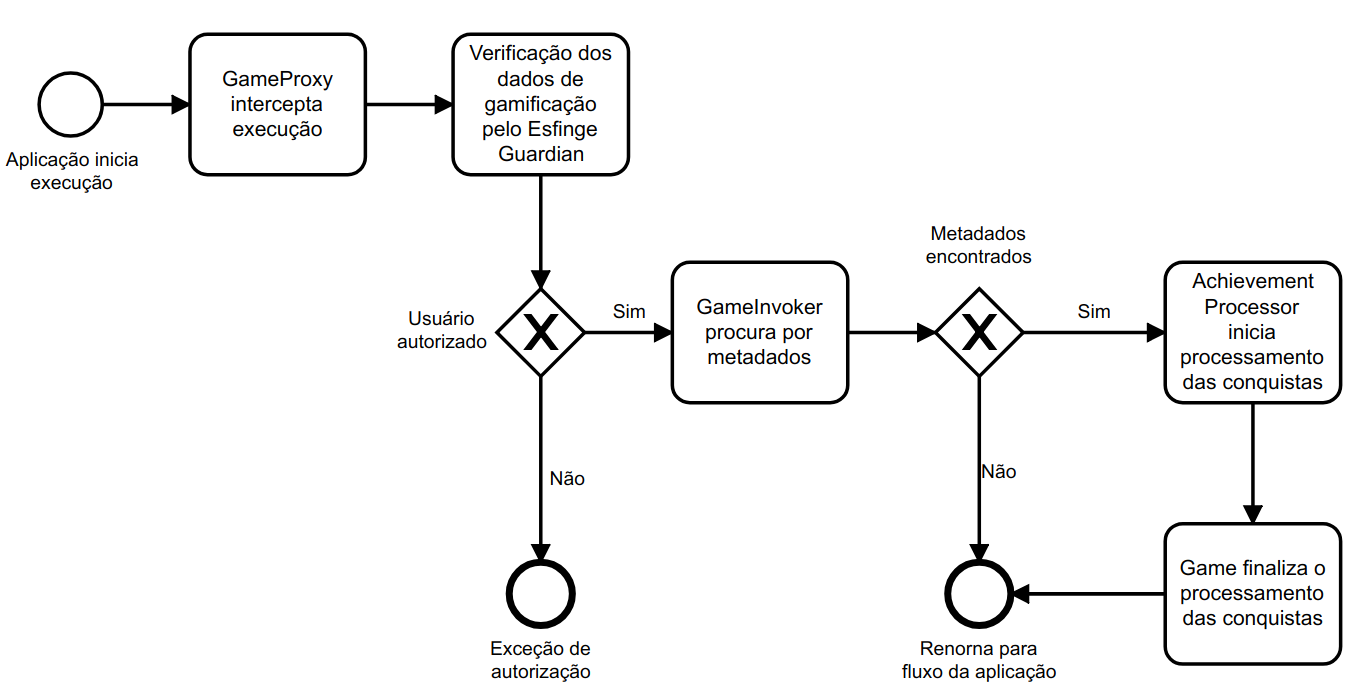
\includegraphics[scale=0.3]{src/imagens/cap3/fluxo-atual.png}
    \caption{Fluxo de funcionamento atual do Esfinge Gamification}
    \label{fig:fluxo-atual}
\end{figure}

Neste fluxo, aplicações em que o Esfinge Gamification foi configurado, são interceptadas via \textit{Proxy} Dinâmico e antes do fluxo de gamificação ser executado o \textit{Proxy} Dinâmico do Esfinge Guardian é invocado para que validações de autorização do usuário sejam realizadas. Na linha 14 da Figura \ref{fig:esfinge-proxy} um objeto que será interceptado pelo Esfinge Guardian é criado, e na linha 8 em que o método recebido pelo Proxy Dinâmico do Esfinge Gamification é invocado o objeto passado como parâmetro para a invocação é o Proxy Dinâmico do Esfinge Guardian, desta forma a responsabilidade de execução é passada para o Esfinge Guardian e as validações ocorrem.

\begin{figure}[H]
    \centering
    \begin{java}
public class GameProxy implements InvocationHandler {

    // Objetos omitidos

    private GameProxy(Object encapsulated) {
                this.encapsulated = encapsulated;
    	// tratativa de excecao omitida
    	this.guardedObject = AuthorizationContext.guardObject(encapsulated);
    	
    }

    public Object invoke(Object proxy, Method method, Object[] args) throws Throwable {
    	try {
        	Object returnValue = method.invoke(guardedObject, args);
        	GameInvoker gameInvoker = GameInvoker.getInstance();
        	gameInvoker.registerAchievment(encapsulated, method, args);
    
    	    return returnValue;
    	} catch (InvocationTargetException e) {
    	    throw e.getTargetException();
    	}
    }
    
    public static <T> T createProxy(T encapsulated) {
    	Object obj = Proxy.newProxyInstance(
                    encapsulated.getClass().getClassLoader(),
                    encapsulated.getClass().getInterfaces(), 
                    new GameProxy(encapsulated)
    	);
    
    	// validacao do Esfinge Metadata validator omitida
    	return (T) obj;
    }
}
    \end{java}
    \caption{Caption}
    \label{fig:esfinge-proxy}
\end{figure}


Após a validação o fluxo de execução é devolvido para o Esfinge Gamification, que procura por metadados e caso alguma implementação da interface \textit{Achievement Processor} for encontrada nos metadados esta é invocada para que os dados de gamificação sejam pré processados. Depois de pré processados os dados são enviados para a especialização escolhida da classe \textit{Game}. Por fim, quando os dados são processados o fluxo é devolvido para a aplicação.

\section{Visão geral}

\par Esta seção tem como objetivo explicar como o framework é usado do jeito mais básico possível, a Figura \ref{fig:hello-world-gamification} realiza a configuração do Esfinge Gamification em um ambiente em que notas podem ser atribuídas a usuários apenas por quem possuir o Ranking \textit{Avaliator} e o Level \textit{Master}. 


\begin{figure}[H]
    \centering
    \begin{java}
    public class AuthorizationSample {
    
	public static void main(String[] args) {

		User user = new User();
		user.setClassroom("C12019");
		user.setRa("C1A252019");
		
		// Metodo de gerencia de conquistas (armazenamento de memoria)
		Game game = new GameMemoryStorage();

		// Configuracao do Esfinge Gamification
		GameInvoker.getInstance().setGame(game);
		UserStorage.setUserID(user.getRa());

		// Cria um objeto para ser monitorado pelo Esfinge Guardian
		User guardedUser = AuthorizationContext.guardObject(user);

		guardedUser.addNote(10.0);

	}
}
    \end{java}
    \caption{Configuração e utilização do \textit{framework}}
    \label{fig:hello-world-gamification}
\end{figure}

Neste exemplo o usuário atual tenta alterar seus pontos e recebe a exceção \textit{"Unauthorized Access"} do pacote \textit{org.esfinge.guardian.exception.AuthorizationException} devido a falta do Ranking necessário, a Figura \ref{fig:execao-configuracao} exibe a configuração realizada na classe \textit{User} para que a autorização seja monitorada pelo Esfinge Guardian.

\begin{figure}[H]
    \centering
    \begin{java}
    public class User {

	private String classroom;
	private String ra;
	private List<Double> notes;

	public User(String classroom, String ra, List<Double> notes) {
		super();
		this.classroom = classroom;
		this.ra = ra;
		this.notes = notes;
	}
    
    // Anotacao de configuracao
	@AllowRankingAndLevel(achievementName = "Avaliator", level = "Master")
	public void addNote(Double note) {
		List<Double> notes = this.getNotes();
		Objects.requireNonNull(notes, "Notes can't be null");
		notes.add(note);
	}
	
	// Getters and setters omitidos
	
	}
    \end{java}
    \caption{Configuração de segurança da classe \textit{User}}
    \label{fig:execao-configuracao}
\end{figure}

\section{Funcionalidades}

\par Para o controle de conquistas as anotações da Tabela \ref{tab:autorizacoes} foram criadas.

\begin{longtable}{|l|m{10cm}|}
\hline
Anotação & Comportamento \\ \hline
\endfirsthead
\endhead
\begin{tabular}[c]{@{}l@{}}
@AllowPointGreaterThan, \\ @AllowPointLessOrEqualsThan, \\ @DenyPointLessOrEqualsThan, \\ @DenyPointGreaterThan
\end{tabular} & Estas anotações verificam se os pontos respeitam as restrições de maior ou menor igual a uma determinada quantidade de pontos definida na anotação para que a autorização seja permitida ou não. \\ \hline
\begin{tabular}[c]{@{}l@{}}
@AllowRanking, \\
@AllowLevel, \\ 
@AllowRankingAndLevel, \\
@AllowRankingOrLevel, \\ 
@DenyLevel, \\
@DenyRanking, \\ 
@DenyRankingAndLevel, \\
@DenyRankingOrLevel
\end{tabular} & As anotações de ranking possuem a mesma lógica das anteriores, porém, visando os recursos do ranking, permitindo e não permitindo o acesso a recursos com as restrições de ranking e level. \\ \hline
@AllowTrophy, @DenyTrophy & Estas anotações verificam o acesso de usuários a recursos protegidos com a restrição de troféu, isto é, quando algum usuário possuir o troféu conseguirá ou não acessar o recurso. \\ \hline
@AllowReward, @DenyReward & Estas anotações verificam o acesso de usuários a recursos protegidos com a restrição de recompensa, isto é, quando algum usuário possuir o recompensa conseguirá ou não acessar o recurso. \\ \hline
\caption{Anotações de autorização}
\label{tab:autorizacoes}\\
\end{longtable}

% ---

% ---
% Incluindo Capitulo 4 - Casos de Testes
\newpage
\chapter{Estudo de caso}

\par Neste capítulo serão apresentados os testes implementados com a solução desenvolvida, a fim de avaliar o funcionamento a partir de duas perguntas de pesquisa (PP):

\begin{itemize}
    \item PP1: O acoplamento entre o \textit{framework} e a aplicação é baixo?
    \item PP2: O \textit{framework} é capaz de realizar o controle de acesso baseado em conquistas?
\end{itemize}

\section{Metodologia}

\par Para o desenvolvimento e testes do estudo de caso é necessário que a aplicação criada possua controle de acesso em funcionalidades, incremento de pontos e adição de Achievements em determinadas situações. Quando algum erro ocorrer mensagens descritivas deverão ser exibidas. Os testes serão avaliados a partir de \textit{logs} da aplicação, onde mensagens de sucesso e falha são exibidos. %O acoplamento entre o \textit{framework} e a aplicação desenvolvida serão analisados a partir de uma matriz de dependência estrutural.

\section{Aplicação desenvolvida}

\par Foi desenvolvida uma aplicação \textit{web}\footnote{O estudo de caso está disponível no endereço https://forum-tg.netlify.com} para utilização dos recursos desenvolvidos, com o objetivo de compartilhamento de ideias e conversas sobre assuntos gerais. Esta aplicação utiliza os mecanismos de pontos e troféus para incentivar a interação entre os usuários, a partir destes mecanismos as regras da Figura \ref{fig:regras-do-forum} foram definidas. Quando usuários conseguem ultrapassar as restrições impostas pelas regras novas funcionalidades são desbloqueadas conforme a utilização da aplicação, e assim, consequentemente, os usuários interagem entre si.

\begin{image}
{0.23}
{src/imagens/cap4/regras-do-forum.png}
{Regras definidas para a aplicação \textit{web}}
{fig:regras-do-forum}
{Produção do autor}
\end{image}

\par Esta aplicação possui o \textit{back-end} hospedado no Heroku\footnote{Heroku é um PaaS que significa \textit{Platform as a Service}. A aplicação está disponível no endereço https://forum-back-end.herokuapp.com}, os próximos testes abordarão os registros da aplicação hospedada no Heroku para confirmar que o Esfinge Guardian realizou as validações esperadas e pode ser utilizado em produção.

\section{Fluxo de funcionamento}

\par O primeiro caso de teste tem como objetivo mostrar que o Esfinge Guardian não interfere no fluxo de funcionamento do Esfinge Gamification quando não há anotações de segurança, permitindo que os recursos de gamificação sejam utilizados normalmente. Para validar essa premissa, um tópico será adicionado com o usuário teste. Quando o usuário acessar seu perfil poderá visualizar que possui agora 10 pontos.

\par Na primeira etapa o usuário teste será criado no \textit{site} para que não possua nenhum ponto, a Figura \ref{fig:ct1-passo1-cadastro} exibe o formulário de cadastro com as informações preenchidas.

\begin{image}
{0.23}
{src/imagens/cap4/ct1/ct1-cadastro-forum.png}
{Cadastro no forum}
{fig:ct1-passo1-cadastro}
{Produção do autor}
\end{image}

\par Após o cadastro realizado, o usuário é redirecionado para a página inicial (Figura \ref{fig:pagina-inicial-apos-cadastro}) e clica em "Criar tópico".

\begin{image}
{0.23}
{src/imagens/cap4/ct1/ct1-tela-incial.png}
{Tela incial após cadastro}
{fig:pagina-inicial-apos-cadastro}
{Produção do autor}
\end{image}

\par Nesta tela, outro formulário é exibido para ser preenchido com as informações relacionadas ao assunto desejado. A Figura \ref{fig:topico-criado} exibe como este formulário foi preenchido.

\begin{image}
{0.23}
{src/imagens/cap4/ct1/ct1-topico-criado.png}
{Primeiro tópico criado pelo usuário teste}
{fig:topico-criado}
{Produção do autor}
\end{image}

\par Após a criação do tópico o usuário é redirecionado para a tela inicial novamente, e seu tópico já está disponível conforme a Figura \ref{fig:tela-inicial-apos-criacao-do-topico} evidencia.

\begin{image}
{0.23}
{src/imagens/cap4/ct1/ct1-tela-incial-com-topico-criado.png}
{Tópico criado pelo usuário teste}
{fig:tela-inicial-apos-criacao-do-topico}
{Produção do autor}
\end{image}

\par A tela do perfil de usuários é exibida quando os botões cinzas com o nome do usuário que criou o tópico são clicados, estes botões ficam disponíveis também em comentários. A Figura \ref{fig:resultado-pontos-apos-criacao-do-topico} confirma a premissa deste teste, exibindo o perfil do usuário teste com 10 pontos após a criação do tópico.

\begin{image}
{0.23}
{src/imagens/cap4/ct1/ct1-resultado.png}
{Resultado obtido após a criação do tópico}
{fig:resultado-pontos-apos-criacao-do-topico}
{Produção do autor}
\end{image}

\par Com as evidências exibidas acima ainda não é possível fazer a identificação de que validações de segurança não foram executadas. Para realizar isto foi preciso verificar os \textit{logs} do servidor. A Figura \ref{fig:ct1-heroku-logs} exibe estes \textit{logs} separados por cores verdes, isto é, a cada linha com o inicio verde onde a data é exibida, um novo \textit{log} foi registrado. O primeiro \textit{log} são registros do clique no botão "Salvar"\ (Figura \ref{fig:topico-criado}), onde uma requisição do tipo POST é feita para que o tópico seja salvo. O segundo \textit{log} é o redirecionamento para a página inicial (Figura \ref{fig:tela-inicial-apos-criacao-do-topico}), onde uma requisição GET é feita para recuperação dos tópicos existentes.

\begin{image}
{0.23}
{src/imagens/cap4/ct1/ct1-heroku-logs.png}
{\textit{Logs} do Heroku não exibindo traços de execução do Esfinge Guardian}
{fig:ct1-heroku-logs}
{Produção do autor}
\end{image}

\par De acordo com o previsto na premissa deste teste o usuário recebeu os 10 pontos após a criação do tópico e o Esfinge Guardian não executou nenhuma validação de segurança.

\section{Incremento dos pontos}

\par Este teste tem como objetivo a validação do incremento dos pontos após a criação de tópicos no \textit{site}, para que as restrições possam ser atingidas e novos recursos desbloqueados. Isto será comprovado a partir do usuário teste utilizado anteriormente, este possui 10 pontos e criará outro tópico, passando a possuir 20 pontos.

\par O mesmo processo realizado na Figura \ref{fig:topico-criado} foi realizado, porém o tópico exibido na Figura \ref{fig:ct2-novo-topico} foi criado.

\begin{image}
{0.23}
{src/imagens/cap4/ct2/ct2-formulario-novo-topico.png}
{Formulário preenchido com novo tópico}
{fig:ct2-novo-topico}
{Produção do autor}
\end{image}

\par Retornando ao perfil do usuário é possível verificar que sua pontuação agora é 20, conforme Figura \ref{fig:ct2-pontuacao-atual}.

\begin{image}
{0.23}
{src/imagens/cap4/ct2/ct2-resultado.png}
{Pontuação do usuário teste}
{fig:ct2-pontuacao-atual}
{Produção do autor}
\end{image}

\par O objetivo deste teste também foi atingido, comprovando o incremento das conquistas permitindo assim que as restrições sejam eliminadas conforme a utilização.

\section{Usuário sem permissão}

\par As restrições serão validadas neste caso de teste, em específico a anotação @AllowPointGreaterThan, que tem como objetivo controlar o acesso de usuários baseando-se em seus pontos, conforme citado na Tabela \ref{tab:autorizacoes}.
\par Quando um usuário possuir menos de 50 pontos, de acordo com as regras do fórum (Figura \ref{fig:regras-do-forum}), este não deve conseguir concluir o processo de atualização do tópico. Para realizar este teste o usuário weslei foi definido, ele possui 10 pontos atualmente, tendo criado apenas um tópico no \textit{site}. O conteúdo do tópico será alterado e uma requisição do tipo PUT será realizada ao servidor para salvar as alterações. O usuário deverá receber a mensagem de erro "Você não possui permissão para atualizar tópicos!"\ devido a falta de pontos.

\par Na Figura \ref{fig:ct3-visualizacao-conteudo} o usuário está na página de visualização detalhada do tópico. É importante ressaltar que os botões "Editar"\ e "Excluir"\ ficam disponíveis apenas para o proprietário do conteúdo. 

\begin{image}
{0.23}
{src/imagens/cap4/ct3/ct3-visualizacao-conteudo.png}
{Tela de visualização detalhada de tópicos}
{fig:ct3-visualizacao-conteudo}
{Produção do autor}
\end{image}

\par Quando o botão "Editar"\ é selecionado os campos do tópico tornam-se editáveis vide Figura \ref{fig:ct3-conteudo-editavel}.

\begin{image}
{0.23}
{src/imagens/cap4/ct3/ct3-conteudo-editavel.png}
{Conteúdo do tópico editável}
{fig:ct3-conteudo-editavel}
{Produção do autor}
\end{image}

\par O botão "Salvar alterações"\ é selecionado pelo usuário e consequentemente uma requisição PUT é feita ao servidor para salvar o conteúdo modificado. As validações são feitas pelo \textit{back-end} e a mensagem de erro "Você não possui permissão para atualizar tópicos!"\ é exibida ao usuário conforme Figura \ref{fig:ct3-mensagem-de-permissao-negada}

\begin{image}
{0.23}
{src/imagens/cap4/ct3/ct3-mensagem-de-permissao-negada.png}
{Mensagem de erro exibida ao realizar processo de edição de tópico sem autorização}
{fig:ct3-mensagem-de-permissao-negada}
{Produção do autor}
\end{image}

\par Seguindo o raciocínio do primeiro teste, apenas a mensagem de erro no \textit{front-end} não é suficiente para validação. Na Figura \ref{fig:processo-autorizacao-gamification} é citada a criação de \textit{logs} durante a validação do Esfinge Guardian. Estes \textit{logs} são criados justamente para identificação de quando acessos a recursos protegidos são feitos. A Figura \ref{fig:log-nao-autorizado} exibe o \textit{log} registrado no momento da requisição inválida realizada pelo usuário weslei, validando o teste.

\begin{image}
{0.15}
{src/imagens/cap4/ct3/ct3-log-nao-autorizado.png}
{\textit{Log} de falta de autorização ao realizar operação de atualização de tópico}
{fig:log-nao-autorizado}
{Produção do autor}
\end{image}

\par Com a criação de \textit{logs} no Esfinge Gamification foi possível confirmar as premissas definidas neste teste, onde o usuário weslei tentou alterar um tópico criado, porém não possuía pontos suficientes para realizar esta operação.

\section{Usuário com permissão}

\par O objetivo deste caso de teste é a autorização, neste caso o processo feito indevidamente no teste anterior será executado novamente com o usuário weslei, porém este possuirá 50 pontos e tentará alterar o mesmo tópico. É esperado que as alterações sejam realizadas com sucesso e que \textit{logs} sejam registrados pelo servidor para confirmação da validação do Esfinge Guardian.

\par Como o incremento das conquistas já foi testado e para agilizar o processo da criação do teste, o ambiente foi alterado para atender este requisito, conforma Figura \ref{fig:pontuacao-weslei} exibe.

\begin{image}
{0.23}
{src/imagens/cap4/ct4/ct4-pontuacao-weslei.png}
{Pontuação do usuário weslei}
{fig:pontuacao-weslei}
{Produção do autor}
\end{image}

\par Novamente o tópico foi selecionado e alterado conforme Figura \ref{fig:ct4-alteracoes-topico}.

\begin{image}
{0.23}
{src/imagens/cap4/ct4/ct4-alteracoes-topico.png}
{Alterações realizadas no tópico}
{fig:ct4-alteracoes-topico}
{Produção do autor}
\end{image}

\par O botão "Salvar alterações"\ é selecionado e o tópico é alterado com sucesso conforme exibido na Figura \ref{fig:ct4-alteracoes-topico}.

\begin{image}
{0.23}
{src/imagens/cap4/ct4/ct4-alteracoes-ok.png}
{Pontuação do usuário weslei}
{fig:ct4-alteracoes-ok}
{Produção do autor}
\end{image}

\par No servidor é possível identificar a verificação realizada pelo Esfinge Guardian. A Figura \ref{fig:ct4-validacao-guardian} exibe os \textit{logs} registrados.

\begin{image}
{0.15}
{src/imagens/cap4/ct4/ct4-validacao-guardian.png}
{Pontuação do usuário weslei}
{fig:ct4-validacao-guardian}
{Produção do autor}
\end{image}

\par Como esperado, o servidor registrou \textit{logs} validando a requisição feita pelo usuário weslei, comprovando que o Esfinge Guardian analisou os dados de gamificação para autorizar a requisição. Um ponto interessante deste \textit{log}, é que a mensagem retornada pelo Esfinge Guardian referente a requisição PUT é exibida antes do \textit{log} da própria requisição, o que pode gerar confusão em um primeiro momento de análise, entretanto o \textit{log} de validação registrado pelo Esfinge Guardian é relativo ao processo de autorização desencadeado pela requisição PUT, realizada pelo usuário weslei.

\section{Matriz de Dependência Estrutural}

\par Matriz de Dependência Estrutural, do inglês \textit{Dependency Structure Matrix} (DSM), tem como objetivo facilitar a visualização entre as dependências do projeto, o acoplamento entre as classes \cite{browning2001applying}. Neste caso o que será abordado é o acoplamento envolvendo a aplicação e o Esfinge Gamification, a partir das Figuras \ref{fig:dsm-configuration-game-setup} e \ref{fig:dsm-service}.

\par A Figura \ref{fig:dsm-configuration-game-setup} exibe o acoplamento envolvendo a configuração do \textit{framework}, esta é realizada na classe GameSetup, presente no pacote br.inpe.forum.gamification. É possível visualizar que esta classe depende de 2 módulos do \textit{framework}: 1) Para criação e interceptação do PD (A); 2) Para definição de persistência de dados (B). Estas dependências são identificadas em amarelo após o nome dos pacotes. Já as classes que dependem de GameSetup são os \textit{controllers} da aplicação, devido a sua responsabilidade, que é a tratativa das requisições.

\begin{image}
{0.27}
{src/imagens/cap4/dsm-configuration-edited-1.png}
{DSM de configuração do \textit{framework}}
{fig:dsm-configuration-game-setup}
{Produção do autor}
\end{image}

\par Este foi o ponto ideal para interceptações, pois quando \textit{controllers} invocam a lógica de negócios na camada de serviço (pacote br.inpe.forum.service), a invocação é interceptada e os metadados definidos nas classes de serviço são lidos pelo \textit{framework}, que realiza o comportamento definido no metadado, conforme exibido nos testes anteriores.

\par A Figura \ref{fig:dsm-service} apresenta a DSM do pacote de serviço, onde as definições de metadados são adicionadas. Como metadados de controle de acesso foram definidos nestas classes, as anotações de segurança (A, B) viram dependências. As dependências C e D existem, pois foi implementado um serviço que recupera dados de gamificação de usuários, portanto é preciso recuperar a instância de Game que é gerenciada pela classe GameProxy (C), e assim recuperar os dados armazenados com a especialização de Game (D).

\begin{image}
{0.27}
{src/imagens/cap4/dsm-service-edited-1.png}
{DSM classes serviço}
{fig:dsm-service}
{Produção do autor}
\end{image}

%\begin{image}
%{0.4}
%{src/imagens/cap4/dsm-classes-forum.png}
%{DSM do projeto desenvolvido}
%{fig:dsm-classes}
%{Produção do autor}
%\end{image}

\par Baseado nas DSMs apresentadas é possível responder a PP1 positivamente, pois o \textit{framework} possui baixo acoplamento com a solução desenvolvida, sendo utilizado apenas em uma classe para configuração, esta é utilizada por classes com responsabilidade de \textit{controller}, para que os métodos possam ser interceptados e pelo serviço responsável por recuperar informações de gamificação de usuários. A principal interface entre o \textit{framework} e a aplicação desenvolvida são as anotações que adicionam os metadados necessários. 
\par A respeito da PP2 é possível concluir que a integração foi um sucesso e que o controle de acesso é eficaz devido aos testes executados nesta seção. Todas as execuções que precisariam ser validadas pelo Esfinge Guardian foram registradas com sucesso pelo servidor a partir de \textit{logs} que confirmaram esta validação. 
\par Desta forma é possível dizer que o Esfinge Gamification é desacoplado de domínio, pode ser facilmente inserido como uma dependência e utilizado em diversas aplicações sem dificuldades, devido a sua generalização.
% ---

% ---
% Incluindo Capitulo 5 - Conclusao
\newpage
\chapter{Conclus\~ao}
\par Conclusao para o trabalho, mostra como a solu\~c\~ao proposta cumpre com o que foi apresentado anteriormente.
% ---

% ---
% Referências bibliográficas
\bibliography{refs/referencias}
% ---
\end{document}
